\begin{figure}[!htbp]
\centering
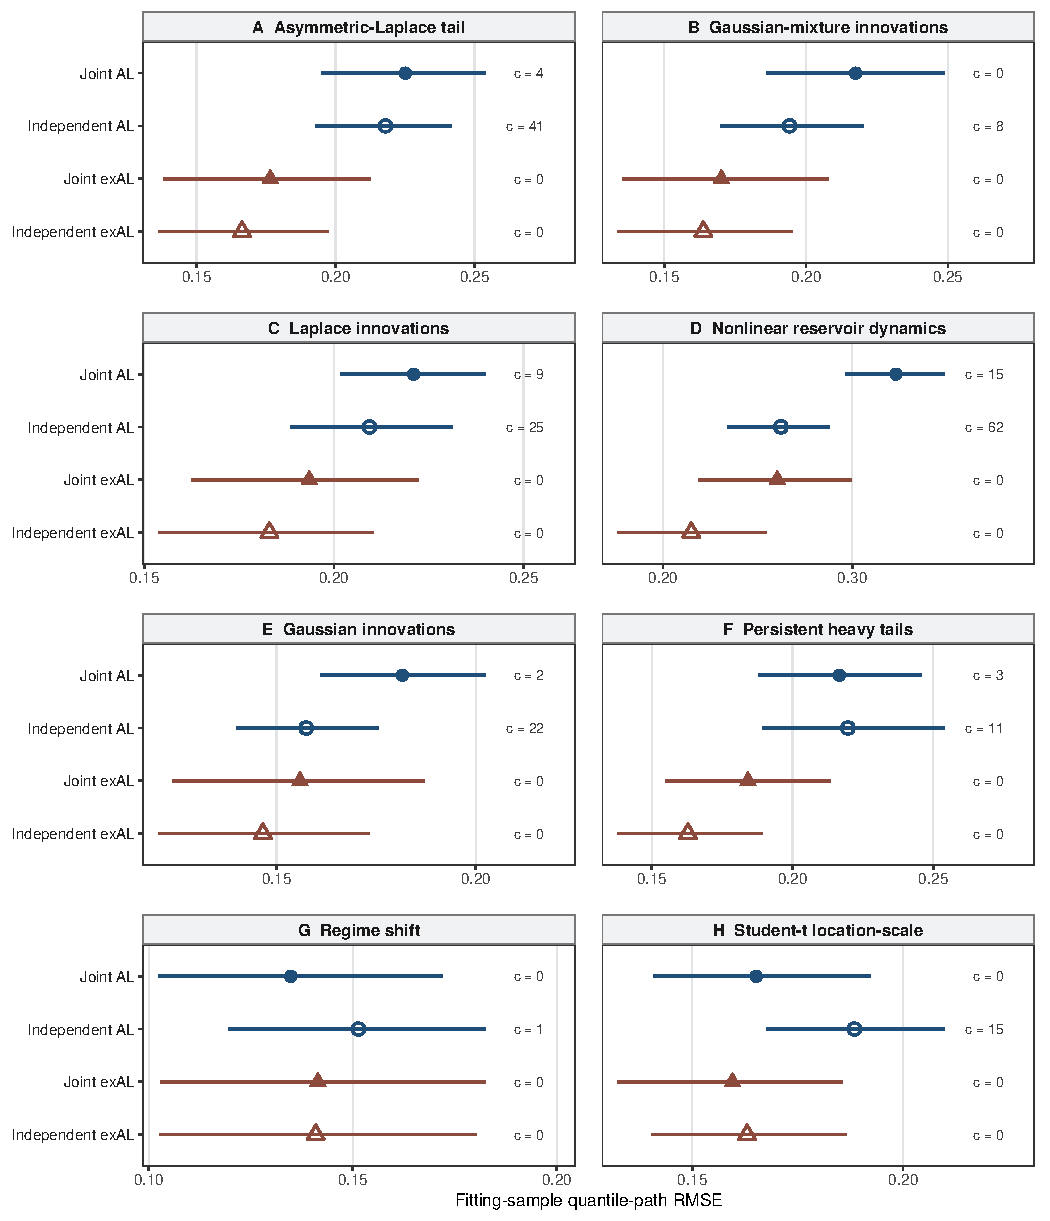
\includegraphics[width=0.94\textwidth]{figures/joint_qdesn_simulation/joint_qdesn_shared_backbone_fit_oracle_rmse_intervals.pdf}
\caption{Posterior fitting-sample recovery of the known conditional quantile
paths under the shared-backbone design. Points are posterior means of
quantile-path RMSE and horizontal segments are equal-tailed 95\% intervals
after monotone rearrangement; lower values are better. Navy circles identify
the \(\AL\) models and muted-brick triangles the \(\exAL\) models; filled
symbols denote joint fits and open symbols independent fits. Panels A--H
identify the data-generating mechanism and use separate horizontal scales.
Labels \(c\) give raw crossings in the posterior-mean grid; all counts after
rearrangement are zero.}
\figalt{Eight panels compare posterior fitting-sample quantile-path RMSE means
and 95 percent intervals for joint and independent AL and exAL models. Each
model is annotated with its number of raw quantile crossings; all rearranged
grids have zero crossings.}
\label{fig:joint-qdesn-shared-backbone-fit-rmse}
\end{figure}
